\documentclass[twoside]{projektInzynierskiMS1}
\usepackage{polski}
\usepackage[utf8]{inputenc}
\usepackage{amsmath}
\usepackage{graphicx}%obrazki
\usepackage{caption}
\usepackage{array,etoolbox}%indeksowanie wierszy w tabelach
\preto\tabular{\setcounter{magicrownumbers}{0}}
\newcounter{magicrownumbers}
\newcommand\rownumber{\stepcounter{magicrownumbers}\arabic{magicrownumbers}}
\usepackage{multirow,tabularx}
\usepackage{etoolbox}
\usepackage{makecell}
\usepackage{float}%obrazki na tej samej stronie
\newcounter{rowcnt}
\newcommand\rownum{\ifnumequal{\value{rowcnt}}{0}{\textbf{Nr.}}{\therowcnt.}\refstepcounter{rowcnt}}
\AtEndEnvironment{tabularx}{\setcounter{rowcnt}{0}}

\captionsetup[table]{aboveskip=0pt}
\captionsetup[table]{belowskip=0pt}

%\drukJednostronny

%% tytuł promotor iautor (\title to komenda standardowa)
\title{Algorytm symulowanego wyżarzania - zastosowanie w rozwiązywaniu zagadnień odwrotnych}
\promotor{dr inż. Adam Zielonka}


%% każdy autor musi mieć 3 argumenty: imię nazwisko, nr albumu, opis wkładu
\autor{Kamil Kryus}{246591}
	


%Custom commands
%-------------------------------------------------------------------------------
\newcommand{\hugeFontSize}{}
\newcommand{\newLine}{~\\}
\newcommand{\si}{ś}
\newcommand{\SI}{Ś}

%-------------------------------------------------------------------------------
%end Custom commands




%\NumeryNaPoczatku
%% numeracja wzorów tu włączona typu (1.2.3), ta druga to typu (1.2), domyślnie typu (1)
%\subsectionWzory
% \sectionWzory  

%\rozdzialy


%\literowaNumeracjaDodatkow %% włączy numerację dodatków literami
%\rzymskaNumeracjaDodatkow  %%włączy numerację dodatków liczbami rzymskimi

%% wyłączenie wyjaśnień:
\bezWyjasnien

%% standardowe komendy \newtheorem  działają jak woryginale
\newtheorem{tw}{Twierdzenie}%[subsection]
\newtheorem{twa}{Twierdzenie}%[section]
\newtheorem{dd}{Definicja}%[subsection]

\begin{document}
Z problematyką wyznaczania optymalnego rozwiązania mamy do czynienia w wielu dziedzinach życia i nauki, np. minimalizując koszty inwestycji, maksymalizując zyski, szukając najkrótszego połączenia pomiędzy miastami itd. Szukając rozwiązania (zazwyczaj przybliżonego), zawsze dążymy do tego, żeby było ono jak ,,najlepsze" (jak najbliższe dokładnemu) i zostało znalezione w rozsądnym czasie. W tym celu można skorzystać z algorytmów heurystycznych. \\ 


Metody heurystyczne są przybliżonymi metodami optymalizacyjnymi, ale otrzymane dzięki nim rezulaty są satysfakcjonujące. Otrzymując w ten sposób rozwiązanie możemy:

\begin{enumerate}
	\item zaakceptować je, np. gdy dokładne rozwiązanie nie jest konieczne np. w kompresji obrazu,
	\item zawęzić (istotnie) zakres i prowadzić dalsze poszukiwania w oparciu o inny algorytm. \\
\end{enumerate}
Metody heurystyczne uznaje się za akceptowalne, jeśli spełniają następujące wymagania:
\begin{itemize}
	\item[--] rozwiązanie jest możliwe do znalezienia przy ,,rozsądnej" liczbie obliczeń,
	\item[--] otrzymane rozwiązanie powinno być bliskie optymalnemu,
	\item[--] prawdopodobieństwo uzyskania złego rozwiązania powinno być ,,niskie".
\end{itemize}

\section{Opis}
Często w naukach technicznych możemy natrafić na zadania, które polegają na odtworzeniu niektórych parametrów modelu na podstawie danych będących wynikiem pewnych obserwacji. W odróżnieniu od bezpo\si rednich problemów, gdzie zaczynając od modelu i danych dochodzimy do rezultatów, w tego typu problemach dzieje się to odwrotnie. Tego typu zadania nazywa się problemami odwrotnymi. \\

Problemy odwrotne niestety są często źle postawione. Problemy, aby być zagadnieniami poprawnie postawionymi, muszą spełniać następujące wymagania:
\begin{enumerate}
	\item rozwiązanie problemu musi istnieć,
	\item każde rozwiązanie jest unikalne,
	\item rozwiązanie zależy od danych oraz parametrów (np. małe zmiany w funkcjach wej\si cia powodują małe zmiany w rozwiązaniu). \\
\end{enumerate}

Jednym z tego typów problemów (problemów odwrotnych) są odwrotne zagadnienia przewodnictwa ciepła. Przy posiadaniu niekompletnego opisu modelu matematycznego oraz funkcji opisującej rozkład temperatury w wybranych punktach (zazwyczaj pomiarowych), zadanie polega na rekonstrukcji brakujących parametrów modelu. 

\subsection{Cel}

W pracy opisany i zaimplementowany zostanie algorytm symulowanego wyżarzania. Dla wybranych funkcji testowych zostały dobrane jego parametry, a finalnie zostanie on wykorzystany do rozwiązania odwrotnego zadania przewodnictwa ciepła.

W tym celu została stworzona w miarę możliwo\si ci uniwersalna aplikacja, która pozwala na znalezienie minimum globalnego funkcjonału, sprawdzona najpierw dla wybranych funkcji testowych, a następnie wykorzystana do odtworzenia brakujących parametrów modelu matematycznego przykładowego odwrotnego zadania przewodnictwa ciepła, przy podanym rozkładzie temperatur w wybranym punkcie pomiarowym.


\section{Opis algorytmu symulowanego wyżarzania}
				Algorytm ten został stworzony wzorując się na zjawisku wyżarzania metali, które polega na nagrzaniu elementu stalowego do ustalonej temperatury początkowej, przetrzymaniu go w tej temperaturze przez ,,pewien" czas, a następnie ,,powolnym" jego schłodzeniu. Sam algorytm natomiast bazuje na metodach Monte-Carlo i w pewnym sensie może być rozważany jako algorytm iteracyjny.\\ \newLine
Główną istotą i zarazem zaletą tego algorytmu jest wykonywanie pewnych ,,losowych przeskoków" do sąsiednich rozwiązań, dzięki czemu jest w stanie uniknąć wpadania w lokalne minimum. Algorytm ten najczę\si ciej jest używany do rozwiązywania problemów kombinatorycznych, takich jak np. problem komiwojażera. \\ \newLine

Zanim jednak przejdziemy do opisu samego algorytmu, powinni\si my najpierw sformułować rozważane zadanie optymalizacyjne.

\subsection{Zadania optymalizacyjne}

Zadania optymalizacyjne polegają na znalezieniu rozwiązania (dokładnego lub zbliżonego) pewnego problemu, zazwyczaj jednak nie jest to możliwe w jednym kroku. Rozwiązanie takiego zadania często wiąże się z pewnym procesem, którego rozwiązanie może być utrudnione np. przez limitowane zasoby mocy obliczeniowej lub inne zdefiniowane warunki. Jednym z typów zadań optymalizacyjnych jest znalezienie minimum globalnego funkcjonału, które można zaprezentować następująco: \\

\begin{alignat*}{2}
f(\overline{x}),&\qquad  x \in D \in R\\
f -> min
\end{alignat*}

		\subsection{Opis algorytmu}
		
\noindent \underline{Początkowa konfiguracja} \\ \newLine
\indent W tym kroku powinniśmy zainicjalizować temperaturę początkową pewną zadaną wartością oraz znaleźć początkowe, w tym wypadku losowe, rozwiązanie problemu. 
\\ \newLine

\noindent \underline{Temperatura} \\ \newLine
\indent  Wraz z upływem czasu (kolejne iteracje) ulega zmianie i jest czynnikiem wpływającym na prawdopodobieństwo zamiany ,,gorszego" rozwiązania na ,,lepsze". Zatem zakres temperatury powinien być taki, aby na początku działania algorytmu dawał dużą możliwość zamian, a wraz z postępem procesu iteracyjnego te prawdopodobieństwo zamiany było bliskie zeru.\\ \newLine

\noindent \underline{Końcowa temperatura} \\ \newLine
\indent Temperatura osiągając taki poziom stanowi, iż proces wyżarzania się zakończył i rozwiązanie zostało znalezione.
Wartość ta powinna być na tyle mała, żeby jej ,,niewielka" zmiana nie miała praktycznego wpływu na zmianę rozwiązania (prawdopodobieństwo zmiany bliskie zeru), a jednocze\si nie jej za mała warto\si ć nie prowadziła do zbyt dużej liczby iteracji. \\ \newLine

\noindent \underline{Powtarzanie zadanej ilo\si ci iteracji dla stałej temperatury} \\ \newLine
Proces iteracyjny bez zmiany temperatury wykonuje się okre\si loną (ustaloną jako parametr algorytmu) ilo\si ć razy. \\ \newLine

\noindent \underline{Znajdowanie losowego sąsiada poprzedniego rozwiązania} \\ \newLine
\indent Funkcja ta powinna nam pozwalać przejrzeć jak najszerszy zakres rozwiązań, a jednocze\si nie pozwolić na przeszukiwanie coraz to bliższych sąsiadów obecnie ,,najlepszego" rozwiązania, zatem funkcję tę należy uzależnić od stopnia zaawansowania procesu iteracyjnego, tak że wraz ze wzrostem iteracji zawężeniu ulegnie obszar przeszukiwania.\\ \newLine

\noindent \underline{Funkcja kosztu} \\ \newLine
\indent Poprzez funkcję kosztu rozumiemy różnicę pomiędzy obecnie najlepszym rozwiązaniem, a nowym. Funkcja ta ma dodatkowe zastosowanie przy decydowaniu o zamianie ,,gorszego" rozwiązania na ,,lepsze". Przy poszukiwaniu globalnego minimum warto\si ć większa jest gorszym rozwiązaniem, dzięki czemu wynikiem tej funkcji jest zawsze liczba ujemna (przy decydowaniu o zamianie). \\ \newLine


\noindent \underline{Prawdopodobieństwo zamiany P} \\ \newLine
\indent Prawdopodobieństwo jest wykorzystywane przy decyzji zamiany nowego i ,,gorszego" rozwiązania, z wcze\si niejszym ,,lepszym". 

Prawdopodobieństwo tej zamiany zależy od funkcji kosztu oraz obecnej temperatury. Prawdopodobieństwo zamiany okre\si lone jest wzorem:
$$ P = \exp\left(\frac{\Delta E}{T}\right),  $$
gdzie:\\
%\begin{flalign}
%& \Delta E&  - funkcja kosztu
%\end{flalign}
$ \Delta E$  - funkcja kosztu, \\
$T$ - obecna warto\si ć temperatury.\\

Prawdopodobieństwo to wraz ze spadkiem warto\si ci funkcji kosztu maleje (gdyż jest zawsze ujemna), natomiast wyższa warto\si ć temperatury zwiększa to prawdopodobieństwo. Decydując o tym, czy powinniśmy zamienić nasze ,,gorsze" rozwiązanie z ,,lepszym", powinniśmy porównać obliczone prawdopodobieństwo z wartością losową o rozkładzie równomiernym.\\ \newLine


\noindent \underline{Chłodzenie temperatury} \\ \newLine
\indent Szybkość chłodzenia temperatury nie powinna być ,,zbyt duża", aby pozwolić algorytmowi na sprawdzenie szerokiego zakresu możliwych rozwiązań, a jednocześnie niezbyt wolna, gdyż może to spowodować zbyt wolny spadek prawdopodobieństwa i zbyt częste akceptowanie ,,gorszych" (lub ,,dużo gorszych") rozwiązań. W większości opracowań można spotkać, że ten proces okre\si la mnożnik tempa spadku temperatury ustalony w zakresie [0.8;0.99].\\ \newLine
		

Z powyższego opisu wynika, że algorytm ten zależy od czterech parametrów:
\begin{itemize}
	\item[--] temperatury początkowej ($T_0$),
	\item[--] temperatury końcowej ($T_{end}$),
	\item[--] wewnętrznych iteracji ($It$),
	\item[--] chłodzenia ($k$).
\end{itemize}

\subsection{Schemat blokowy}
Przygotowali\si my również schemat blokowy reprezentujący poszczególne kroki i scenariusze w procesie poszukiwania rozwiązania zadanego problemu, co można zobaczyć na poniższym rysunku.

\begin{figure}[H]
		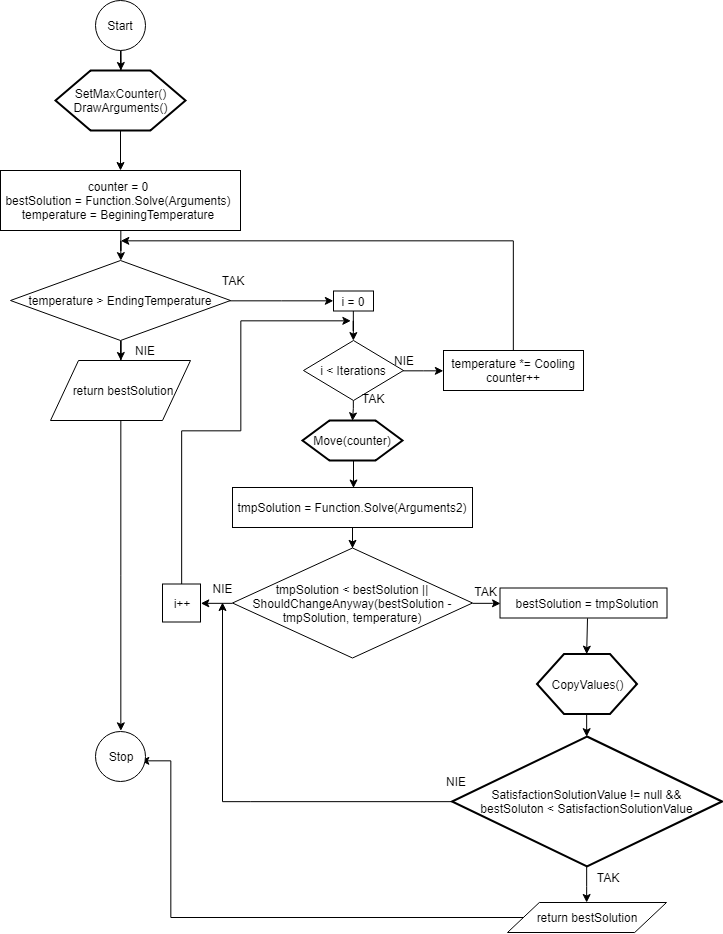
\includegraphics[height=22cm, width=16cm]{pics/blockDiagram.png}\\
	\caption{Schemat blokowy algorytmu symulowanego wyżarzania}
\end{figure}


		\subsection{Kroki algorytmu}
		
		Algorytm ten można przedstawić schematycznie:

\begin{enumerate}
	\item Inicjalizacja $T_{0}$, $T_{end}$, $It$, $k$
	\item T = $T_{0}$
	\item $x_{best}$ = losowe współrzędne z dziedziny zadania
	\item Dopóki T $>$ $T_{end}$:
	
	\begin{enumerate}
		\item  Wyznacz ,,sąsiada" współrzędnych $x_{best}$ (wraz z liczbą iteracji szeroko\si ć zakresu wyznaczania ,,sąsiada" maleje, zmienna $x_{tmp}$)
		\begin{enumerate}
			\item[I.] Je\si li f($x_{best}$) $>$ f($x_{tmp}$):
			\begin{enumerate}
				\item $x_{best}$ = $x_{tmp}$
			\end{enumerate}
			\item[II.] w przeciwnym wypadku:
			\begin{enumerate}
				\item $\Delta E$ = f($x_{best}$) - f($x_{tmp}$)
				\item $P$ = $\exp\left(\frac{\Delta E}{T}\right)$
				\item $q$ = losowa liczba z przedziału [0, 1]
				\item Je\si li $P$ $>$ $q$, to:
				\begin{itemize}
					\item[i.] $x_{best}$ = $x_{tmp}$
				\end{itemize}
			\end{enumerate}
			\item Wróć do (a) $It$ razy
		\end{enumerate}
		\item $T$ = $k$$T$
		\item Wróć do 4.
	\end{enumerate}	
\end{enumerate}
	

\section{Narzędzia i technologie}
W procesie tworzenia aplikacji zdecydowali\si my się na użycie kilku rozwiązań, które pozwoliły na bezpieczną i przejrzystą pracę w kolejnych jego etapach. \\
	\subsection{Metodyka pracy}
	\subsubsection{System kontroli wersji}
	System kontroli wersji posiada wiele zalet, m.in.: bezpieczeństwo, możliwo\si ć pracy w kilku miejscach/urządzeniach nad tym samym problemem, łatwą możliwo\si ć przywrócenia poprzedniej wersji, czy wreszcie, inspekcję jako\si ci i poprawno\si ci kodu. \\
W moim projekcie skorzystałem z systemu kontroli Git, a repozytorium można znaleźć na portalu github.com. 
	\subsubsection{Github Project Management}
Pomimo, iż praca w pojedynkę nie wymagała ode mnie zaawansowanego zarządzania projektem i konieczno\si ci organizacji pracy, zdecydowałem się na użycie narzędzia pozwalającego na taką pracę. Podzielenie projektu na mniejsze zadania pozwoliło mi wydzielić poszczególne i odrębne sektory pracy, widzieć postępujący progres i łatwo odnaleźć się w aktualnie wykonywanym zadaniu. W tym celu skorzystałem z Github Project Management, który pozwala na proste zarządzanie zadaniami.
	\subsubsection{Środowisko programistyczne}
Do implementacji projektu użyłem \si rodowiska Microsoft Visual Studio Community 2017, które to zostało stworzone przez firmę Microsoft i pozwala na programowanie konsolowe oraz z graficznym interfejsem użytkownika (zarówno aplikacje desktopowe, jak i strony internetowe).  \\
Dobra znajomo\si ć i przejrzysto\si ć tego \si rodowiska programistycznego pozwoliła mi skupić się na rozwiązywaniu problemu, omijając problem zapoznawania się z nowym narzędziem.
	\subsubsection{Mathematica}
	Mathematica jest programem opartym na systemie obliczeń symbolicznych oraz numerycznych. Program ten jest do\si ć popularny w\si ród naukowców ze względu na wiele zalet, jak np. wydajno\si ć czy rozpięte możliwo\si ci wizualizacji danych. Mathematica jest programem komercyjnym, dlatego stworzenie wykresów do tego projektu oparłem na licencji wydziału Matematyki Stosowanej.
	
	\subsection{Użyte technologie}
	\subsubsection{C\#}
Język programowania C\# należy do obiektowych języków programowania, którego koncepcja opiera się na tworzeniu klas, które poprzez swoją zawarto\si ć (m.in. wła\si ciwo\si ci czy metody) mogą być reprezentowane poprzez obiekty i każde operacje są wykonywane poprzez nie. W projekcie korzystam z języka C\# w wersji 7.0, która w momencie rozpoczęcia pracy była aktualna. Dobra znajomo\si ć tego języka pozwoliła mi nie zważać na problemy w znajomo\si ci składni czy funkcji i skupić się bezpo\si rednio na implementacji algorytmów, dobraniu odpowiednich parametrów dla poszczególnych funkcji testowych oraz lepszym przetestowaniu całej funkcjonalno\si ci.

\subsubsection{Wolfram Language}
Język ten służy głównie do programowania obliczeń matematycznych i programowania funkcjonalnego w programie Mathematica. Język ten, wraz z oprogramowaniem Mathematica, pozwalają m.in. na: operacje na macierzach, rozwiązywanie równań różniczkowych czy prezentowanie danych za pomocą wykresów. Z tej ostatniej funkcjonalno\si ci skorzystałem tworząc wykresy funkcji testowych.

\section{Funkcje testowe}
Pomimo, iż algorytmy heurystyczne są dobrym wyborem wszędzie tam, gdzie brak jest informacji o funkcji, a jedynie znane są jej warto\si ci, to przed użyciem danego algorytmu musimy dobrać parametry algorytmu w taki sposób, by wynik był dostatecznie dokładny, a algorytm nie wykonywał niepotrzebnie obliczeń, zwłaszcza gdy większa dokładno\si ć nie jest nam potrzebna lub nie będzie stanowić większej różnicy w stosunku do już znalezionego wyniku. Dodatkową trudno\si ć stanowi ilo\si ć parametrów oraz to, iż każdy z nich może wpływać w inny sposób na złożono\si ć obliczeniową oraz wynik. W opracowaniach naukowych trudno znaleźć wytyczne co do sposobu wyznaczania odpowiednich parametrów, związane to jest z ich zależno\si cią od rozwiązywanego problemu. \\




W pierwszej kolejno\si ci został przeprowadzony test dla szerokiego zakresu każdego z parametrów i że względu na dużą ilo\si ć prób, wykonano po 10 powtórzeń algorytmu dla tych samych parametrów algorytmu. W ten sposób uzyskali\si my ,,obiecujące" zestawy parametrów wyj\si ciowych algorytmu i następnie dla nich zostały przeprowadzone próby, gdzie wykonano po 100 powtórzeń algorytmu dla tych samych, wyselekcjonowanych parametrów. W przypadku funkcji testowej Rastrigina w $R^5$ proces wyznaczania parametrów zostanie opisany dokładnie, a w pozostałych przypadkach zostały zamieszczone wyselekcjonowane parametry algorytmu.



	\subsection{Funkcja kwadratowa dwóch zmiennych}
	Jako pierwszą funkcję do testów przyjęli\si my funkcję kwadratową dwóch zmiennych postaci:
\begin{alignat*}{2}
f(x, y) = x^2 + y^2,&\qquad  (x, y) \in R^2\\
\end{alignat*}

Wybór tak ,,łatwej" funkcji testowej padł ze względu na to, żeby upewnić się, że algorytm został poprawnie zaimplementowany, gdyż proces wyznaczania ekstremum tej funkcji jest ,,bardzo prosty" i nie wymaga dużego nakładu obliczeń. \\

Funkcja ta przyjmuje tylko warto\si ci nieujemne i posiada minimum globalne w punkcie (0, 0). Na potrzeby testów dziedzina tej funkcji została zawężona następująco:
\[(x, y)  \in [0,1]^2 \]\\ 


Funkcję prezentuje poniższy wykres:\\
\begin{figure}[H]
	\begin{center}
		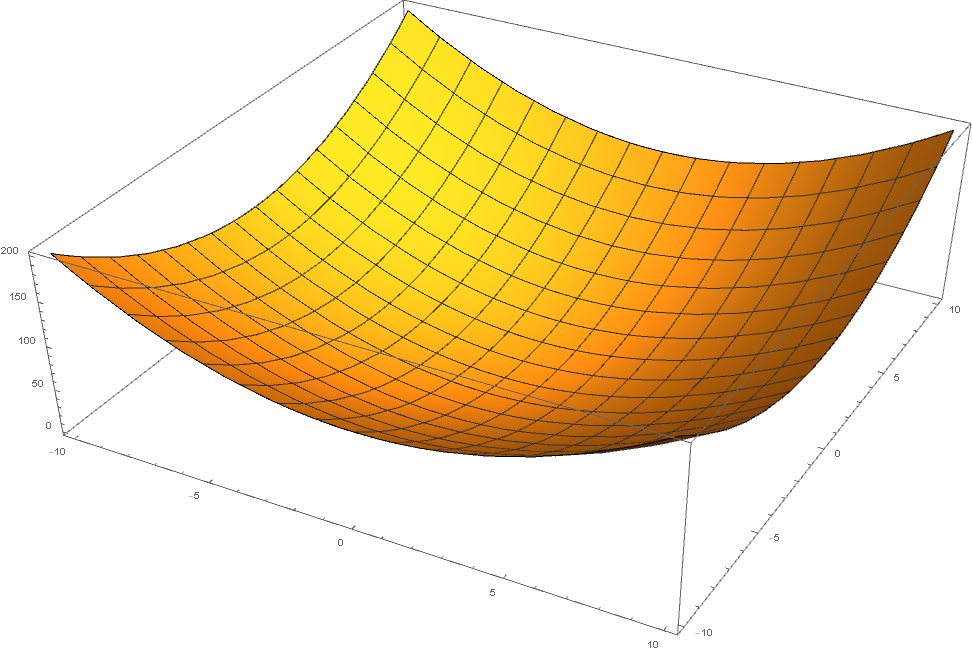
\includegraphics[height=7cm]{pics/quadraticFunction1.png}\\
	\end{center}
	\caption{Funkcja kwadratowa dwóch parametrów}
\end{figure}

	\subsubsection{Parametry dobrane dla funkcji kwadratowej dwóch parametrów}
Poniższa tabela przedstawia parametry pozwalające na znalezienie rozwiązania z satysfakcjonującą jako\si cią:\\

\begin{tabularx}{\textwidth}{ |X|X|} 
\hline
 \textbf{ Parametr} & \textbf{ Warto\si ć}\\ \hline
 $T_0$ & 1\\ \hline 
 $T_{end}$ & 0.01 \\ \hline
$It$ & 1 \\ \hline  
 $k$& 0.99 \\ \hline 

 Skuteczno\si ć & 100\% \\ \hline 
\end{tabularx} \\
 
	\subsection{Funkcja Rastrigina}
	Funkcja Rastrigina jest funkcją ciągłą, skalowalną i multimodalną (dla n=2, została przedstawiona na rysunku 2). Dzięki posiadaniu wielu minimum lokalnych, funkcja ta jest często stosowana w testowaniu algorytmów optymalizacyjnych. Przyjmuje ona następującą postać:

\[f(x) = An + \sum_{i=1}^{n} [x_i^2 - A \cos{\left(2 \pi x_i\right)}] \]

\noindent gdzie: \\
A = 10, \\
n = ilo\si ć wymiarów. \\ \newLine

\begin{figure}[H]
	\begin{center}
		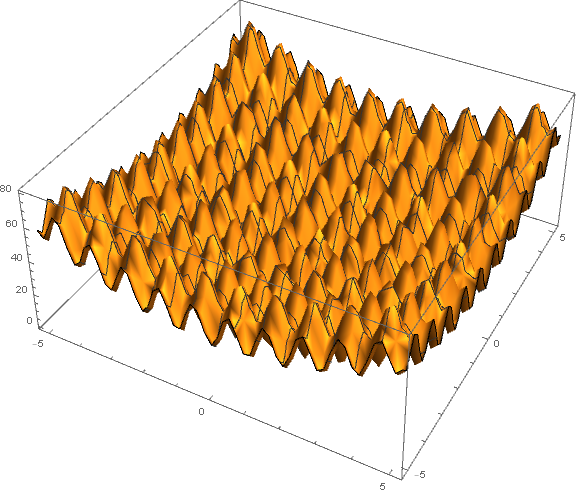
\includegraphics[height=7cm]{pics/rastriginFunction1.png}\\
	\end{center}
	\caption{Funkcja Rastrigina o 2 wymiarach}
\end{figure}

Warto\si ci tej funkcji są nieujemne. Zakres warto\si ci dla tej funkcji znajdziemy w przedziale:
\[x_i \in [-5.12, 5.12] \] \\

Posiada ona następujące globalne minimum:
\[ f(0,...,0) = 0 \] \\


	\subsubsection{Dobieranie parametrów dla funkcji Rastrigina o 3 wymiarach}
Po przeprowadzeniu testów zostały dobrane następujące parametry: \\

\begin{tabularx}{\textwidth}{ |X|X|} 
\hline
 \textbf{ Parametr} & \textbf{ Warto\si ć}\\ \hline
 $T_0$ & 10 \\ \hline 
 $T_{end}$ & 0.01 \\ \hline 
 $It$ & 600 \\ \hline 
$k$& 0.99 \\ \hline 
 Skuteczno\si ć & 100\% \\ \hline 
\end{tabularx} \\

\subsubsection{Dobieranie parametrów dla funkcji Rastrigina o 5 wymiarach}

Przed rozpoczęciem testów przyjęto dwa założenia:
\begin{enumerate}
	\item Końcowa temperatura została ustawiona na stałą warto\si ć równą 0.01,
	\item Stopień chłodzenia temperatury został ustawiony na 0.99.
\end{enumerate}

W pierwszym etapie została sprawdzona temperatura w zakresie (2, 4, ..., 10) oraz ilo\si ć iteracji w liczbie (100, 300, ..., 1100). \\
\begin{table}[htbp]\centering
\def\sym#1{\ifmmode^{#1}\else\(^{#1}\)\fi}
\caption{Wyniki testów parametrów dla podanych zakresów, gdzie $T_0$ jest temperaturą początkową, $It$ jest ilo\si cią iteracji, a $\overline{f}_{min}$ \si rednią rozwiązań dla podanych parametrów}
%\footnotesize Smaller note of table that describes what the table is all about.
\renewcommand\arraystretch{1.333}
\begin{tabular}{|c|c|c||c|c|c|} 
                  \hline
                  $T_0$
                  & $It$
                  & $\overline{f}_{min}$ 
& $T_0$
 & $It$
 & $\overline{f}_{min}$ \\ \hline

10 & 1100 & 1,6194 &4 & 1100 & 1,8291 \\ \hline
10 & 900 & 1,7176 &4 & 900 & 1,5182 \\ \hline
10 & 700 & 1,4182&4 & 700 & 2,3089 \\ \hline
10 & 500 & 1,8106&4 & 500 & 2,2251 \\ \hline
10 & 300 & 1,8099 &4 & 300 & 2,5146 \\ \hline 
10 & 100 & 2,8057&4 & 100 & 3,2157 \\ \Xhline{3\arrayrulewidth}

8 & 1100 & 1,4151 &2 & 1100 & 1,8087 \\ \hline 
8 & 900 & 1,5191 &2 & 900 & 2,2128 \\ \hline 
8 & 700 & 1,6145 &2 & 700 & 1,9127 \\ \hline
8 & 500 & 1,6169 &2 & 500 & 1,5137 \\ \hline 
8 & 300 & 2,4199 &2 & 300 & 2,3170 \\ \hline 
8 & 100 & 3,2014 &2 & 100 & 3,0159 \\ \Xhline{3\arrayrulewidth}

6 & 1100 & 1,3214 \\ \hline 
6 & 900 & 1,3201 \\ \hline 
6 & 700 & 1,8174 \\ \hline 
6 & 500 & 1,5151 \\ \hline 
6 & 300 & 2,0083 \\ \hline 
6 & 100 & 3,0047 \\ \hline 
\end{tabular}
\end{table}

Powyższe wyniki nie dają zadowalających rezultatów. Można jednak zauważyć, iż w tym momencie badań temperatura nie ma aż takiego znaczenia, a większa ilo\si ć iteracji zdaje się dawać lepsze rezultaty. Zgodnie z założeniem, iż temperatura nie powinna być zbyt wysoka, postanowili\si my dalej sprawdzać ten sam zakres temperatur i zwiększyć ilo\si ć iteracji około stukrotnie, co prezentuje następna tabela.


\begin{tabular}{|c|c|c|} 
                  \hline
                   $T_0$
                  & $It$ (*1000)
                  &$\overline{f}_{min}$\\ \hline


10 & 11 & 0,7165\\ \hline 
10 & 9 & 0,8208 \\ \hline 
10 & 7 & 1,3270 \\ \hline 
10 & 5 & 0,8244 \\ \hline 
10 & 3 & 1,5143 \\ \hline 
10 & 1 & 1,3252 \\ \Xhline{3\arrayrulewidth}

8 & 11 & 0,8120 \\ \hline 
8 & 9 & 1,0224 \\ \hline 
8 & 7 & 1,0155 \\ \hline 
8 & 5 & 1,3222 \\ \hline 
8 & 3 & 1,2153 \\ \hline 
8 & 1 & 1,6182 \\ \Xhline{3\arrayrulewidth}


6 & 11 & 0,9273 \\ \hline 
6 & 9 & 0,7189 \\ \hline 
6 & 7 & 0,7157 \\ \hline 
6 & 5 & 1,3202 \\ \hline 
6 & 3 & 1,3194 \\ \hline 
6 & 1 & 1,3147 \\ \Xhline{3\arrayrulewidth}


4 & 11 & 1,1203 \\ \hline 
4 & 9 & 0,9278 \\ \hline 
4 & 7 & 1,3136 \\ \hline 
4 & 5 & 0,9184 \\ \hline 
4 & 3 & 1,0177 \\ \hline 
4 & 1 & 1,5184 \\ \Xhline{3\arrayrulewidth}

2 & 11 & 0,5162 \\ \hline 
2 & 9 & 1,1158 \\ \hline 
2 & 7 & 1,3152 \\ \hline 
2 & 5 & 0,9171 \\ \hline 
2 & 3 & 1,3114 \\ \hline 
2 & 1 & 1,4161 \\ \Xhline{3\arrayrulewidth}


\end{tabular} \\

Średnia rozwiązań najlepszego wyniku w tym te\si cie wydawała się być obiecująca, jednak sprawdzenie jako\si ci takich parametrów zwróciło jako\si ć równą 34\%, co jest niskim wynikiem. Postanowili\si my zwiększyć znowu zakres iteracji dziesięciokrotnie, co można zobaczyć w następnej tabeli.

\begin{table}[htbp]\centering
\def\sym#1{\ifmmode^{#1}\else\(^{#1}\)\fi}
\caption{Wyniki testów parametrów dla podanych zakresów, gdzie $T_0$ jest temperaturą początkową, $It$ jest ilo\si cią iteracji, a $\overline{f}_{min}$ \si rednią rozwiązań dla podanych parametrów}
%\footnotesize Smaller note of table that describes what the table is all about.
\begin{tabular}{|c|c|c||c|c|c|} 
                  \hline
                   $T_0$
                  & $It$ (*1000)
                  &$\overline{f}_{min}$ 
& $T_0$
 & $It$ (*1000)
 &$\overline{f}_{min}$ \\ \hline
10 & 100 & 0,1215 & 4 & 100 & 0,2337 \\ \hline
10 & 90 & 0,0252 & 4 & 90 & 0,3147 \\ \hline
10 & 80 & 0,1216 & 4 & 80 & 0,2206 \\ \hline
10 & 70 & 0,3249& 4 & 70 & 0,2209 \\ \hline 
10 & 60 & 0,3199 & 4 & 60 & 0,2178 \\ \hline 
10 & 50 & 0,5257 & 4 & 50 & 0,3222 \\ \hline
10 & 40 & 0,5223 & 4 & 40 & 0,5243 \\ \hline 
10 & 30 & 0,8243 & 4 & 30 & 0,5192 \\ \hline
10 & 20 & 0,3277 & 4 & 20 & 0,3261 \\ \hline 
10 & 10 & 0,5312 & 4 & 10 & 0,7265 \\ \Xhline{3\arrayrulewidth}

8 & 100 & 0,2279 & 2 & 100 & 0,3224 \\ \hline 
8 & 90 & 0,4161 & 2 & 90 & 0,6167 \\ \hline 
8 & 80 & 0,2257 & 2 & 80 & 0,2266 \\ \hline 
8 & 70 & 0,2200 & 2 & 70 & 0,3247 \\ \hline 
8 & 60 & 0,6255 & 2 & 60 & 0,5264 \\ \hline 
8 & 50 & 0,4257 & 2 & 50 & 0,3248 \\ \hline 
8 & 40 & 0,1310 & 2 & 40 & 0,4396 \\ \hline
8 & 30 & 0,5167 & 2 & 30 & 0,6237 \\ \hline
8 & 20 & 0,8323 & 2 & 20 & 0,4180 \\ \hline
8 & 10 & 1,1295 & 2 & 10 & 0,8205 \\ \Xhline{3\arrayrulewidth}

6 & 100 & 0,2208 \\ \hline 
6 & 90 & 0,2242 \\ \hline 
6 & 80 & 0,5203 \\ \hline 
6 & 70 & 0,8194 \\ \hline 
6 & 60 & 0,5308 \\ \hline 
6 & 50 & 0,4199\\ \hline 
6 & 40 & 0,3182 \\ \hline 
6 & 30 & 0,4311 \\ \hline 
6 & 20 & 0,5213 \\ \hline 
6 & 10 & 0,7173 \\ \Xhline{3\arrayrulewidth}


\end{tabular} 
\end{table}

Otrzymane wyniki sugerują, iż najlepsze wyniki dla podanych zakresów można otrzymać przy temperaturze równej 10 i bardzo wysokich ilo\si ciach iteracji. W następnym kroku sprawdzili\si my jako\si ć rozwiązań dla temperatury równej 10 i iteracji w zakresie przedstawionej w tabeli. \\

\begin{tabularx}{\textwidth}{|X|X|X|} 
                  \hline
 \textbf{ $T_0$} & \textbf{Iteracje (*1000)}& \textbf{ Jako\si ć [\%]}\\ \hline
10 & 10 & 29 \\ \hline
10 & 20 & 42 \\ \hline
10 & 30 & 45 \\ \hline 
10 & 40 & 57 \\ \hline 
10 & 50 & 69 \\ \hline 
10 & 60 & 66 \\ \hline
10 & 70 & 68 \\ \hline 
10 & 80 & 74 \\ \hline 
10 & 90 &  80\\ \hline 
10 & 100 & 81 \\ \hline 
\end{tabularx} \\

Jako\si ć rzędu 75-80\% wydaje się być zadowalająca, dlatego uznali\si my, że proces poszukiwania parametrów dla algorytmu symulowanego wyżarzania dla tego problemu został zakończony. Kolejna tabela przedstawia ostatecznie wybrane parametry dla tego problemu. \\

\begin{tabularx}{\textwidth}{ |X|X|} 
\hline
 \textbf{ Parametr} & \textbf{ Warto\si ć}\\ \hline
 $T_0$ & 10 \\ \hline 
 $T_{end}$ & 0.01 \\ \hline 
 $It$ & 90000 \\ \hline
 $k$& 0.99 \\ \hline 
 Skuteczno\si ć & 80\% \\ \hline 
\end{tabularx}


	\subsection{Funkcja Rosenbrocka}
Funkcja ta jest funkcją ciągłą, skalowalną i jednomodalną (chociaż niektóre źródła podają, że w większej ilo\si ci wymiarów może być multimodalną\footnote{Y. Shang, Y. Qiu, \textit{A Note on the Extended Rosenbrock Function} https://www.mitpressjournals.org/doi/abs/10.1162/evco.2006.14.1.119 [Dostęp: 7 listopada 2018]}).

%\[f(x) = \sum_{i=1}^{n-1} [100\left(x_{i+1} - x_i^2\right)^2 + \left(1- x_i\right)^2 ]\] \\


\begin{alignat*}{2}
f(x) = \sum_{i=1}^{n-1} \left[100\left(x_{i+1} - x_i^2\right)^2 + \left(1- x_i\right)^2\right],&\qquad  x_i \in R\\
\end{alignat*}

Funkcja ta również przyjmuje wyłącznie warto\si ci nieujemne. Na potrzeby projektu warto\si ci argumentów dla tej funkcji zostały zawężone do poniższego zakresu:
\[x_i \in [-10, 10] \] \\

Posiada ona następujące globalne minimum:
\[ f(1,...,1) = 0 \] \\

Poniższy wykres prezentuje jej wygląd w zadanym zakresie:\\
\begin{figure}[H]
	\begin{center}
		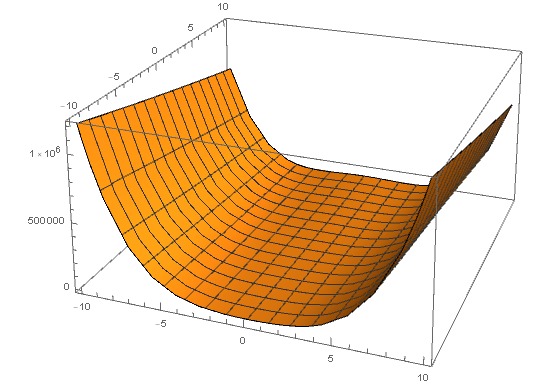
\includegraphics[height=7cm]{pics/rosenbrockFunction1.png}\\
	\end{center}
	\caption{Funkcja Rosenbrocka o 2 wymiarach}
\end{figure}

	\subsubsection{Parametry dobrane dla funkcji Rosenbrocka o 3 wymiarach}
Poniższa tabela przedstawia parametry, które pozwalały na uzyskanie satysfakcjonującego rozwiązania z dostatecznie ,,dużą" pewno\si cią ich otrzymania: \\

\begin{tabularx}{\textwidth}{ |X|X|} 
\hline
 \textbf{ Parametr} & \textbf{ Warto\si ć}\\ \hline
 $T_0$ & 10 \\ \hline 
 $T_{end}$ & 0.01 \\ \hline 
 $k$& 0.99 \\ \hline 
 $It$ & 500 \\ \hline 
 Skuteczno\si ć & 100\% \\ \hline 
\end{tabularx}

\section{Implementacja}

Algorytm symulowanego wyżarzania składa się z kilku metod, które zostały przedstawione w rozdziale 2.1.2. W rozdziale tym skupimy się na omówieniu tych metod oraz przedstawimy ich implementację w języku C\#. \\

\subsection{Używane parametry i zmienne}
Wraz z zainicjalizowaniem obiektu symulowanego wyżarzania, należy ustawić parametry (XXX)
 na wej\si cie, a konkretniej problem do rozwiązania i parametry samego algorytmu. W programie zostały one nazwane: \textbf{Function}, \textbf{Arguments}, \textbf{Arguments2}, \textbf{Iterations}, \textbf{BeginingTemperature}, \textbf{EndingTemperature}, \textbf{Cooling}, \textbf{SatisfactionSolutionValue}. \\

\textbf{Function} jest identyfikatorem referencji do obiektu reprezentującego problem. Każdy problem musi dziedziczyć po klasie abstrakcyjnej ,,TestingFunction", co zapewnia uniwersalno\si ć stosowania algorytmu symulowanego wyżarzania oraz zapewnia nasz algorytm, iż implementacja samego problemu będzie posiadać pewne cechy (jak np. jawnie okre\si loną ilo\si ć wymiarów). \\

\textbf{Arguments} jest wła\si ciwo\si cią w postaci tablicy liczb zmiennoprzecinkowych, która reprezentuje współrzędne dla obecnie najlepszego rozwiązania problemu ($x_{best} = (x_1, x_2, ..., x_n)$). \\

\textbf{Arguments2} jest również tablicą liczb zmiennoprzecinkowych, jednak przechowuje ona współrzędne dla tymczasowego rozwiązania. Jest tego samego rozmiaru, co wła\si ciwo\si ć \textbf{Arguments} ($x_{tmp} = (x_1, x_2, ..., x_n)$). \\

\textbf{BeginingTemperature} jest to początkowa warto\si ć temperatury, od której rozpoczyna się proces poszukiwań rozwiązania. \\ 

\textbf{EndingTemperature} jest liczbą, którą obniżana temperatura (zmienna \textbf{temperature}) musi osiągnąć, by zakończyć działanie algorytmu. \\

\textbf{Iterations} jest liczbą wewnętrznych iteracji (ilo\si ć powtórzeń algorytmu bez obniżania temperatury). \\

\textbf{Cooling} to liczba zmiennoprzecinkowa, w każdym głównym kroku algorytmu zmienna \textbf{temperature} jest mnożona przez tą warto\si ć. Jest ona z przedziału (0, 1), więc temperatura powoli się obniża. \\

\textbf{SatisfactionSolutionValue} jest liczbą, jaką rozwiązanie musi osiągnąć, aby wynik poszukiwania rozwiązania był dla nas satysfakcjonujący. Jest to zmienna opcjonalna, algorytm nadal będzie działać, gdy nie poda się jej warto\si ci. Dzięki niej, je\si li funkcjonał osiągnie warto\si ć oczekiwaną, to przestaje działać algorytm.\\

W programie również używam kilku pomocnicznych zmiennych: \\

\textbf{temperature} to zmienna, która reprezentuje temperaturę. Jest ona używana w warunkach głównej iteracji oraz do wyznaczania funkcji prawdopodobieństwa. Wraz z postępem iteracji maleje. \\

\textbf{bestSolution} to liczba zmiennoprzecinkowa, która reprezentuje warto\si ć obecnie najlepszego rozwiązania. Finalnie będzie ona warto\si cią funkcjonału dla najlepszego rozwiązania całego problemu. \\

\textbf{tmpSolution} jest tymczasowym wynikiem rozwiązania (wynikiem rozwiązania problemu dla parametrów ze zmiennej \textbf{Arguments2}). \\

\textbf{counter} jest liczbą oznaczającą miarę głównej iteracji. \\

\subsection{Implementacja metod i algorytmu}

\underline{Metoda SetMaxCounter()} \\
Metoda ta symuluje proces obniżania temperatury w celu obliczenia maksymalnej ilo\si ci głównych iteracji. \\
\begin{verbatim}
private void SetMaxCounter()
{
    maxCounter = 0;
    double tmpTemperature = BeginingTemperature;
    while (tmpTemperature > EndingTemperature)
    {
        tmpTemperature *= Cooling;
        maxCounter++;
    }
}
\end{verbatim}

\underline{Metoda DrawArguments()} \\
W metodzie tej losuję początkowe argumenty (wła\si ciwo\si ć \textbf{Arguments}) z przedziału zadanego dla danego zagadnienia. \\\


%

\underline{Metoda Move()} \\
W tym miejscu najpierw obliczany jest pozostały procent iteracji do ukończenia procesu (znając parametry algorytmu można wyznaczyć ilo\si ć głównych iteracji). Następnie biorąc 80\% szeroko\si ci zakresu warto\si ci ze zmiennych (zmienna partOfTheDomain), mnożymy ją przez pozostały do końca procesu procent iteracji (i przypisujemy do zmiennej value). Dalej, w pętli, każdej składowej tymczasowego rozwiązania (wła\si ciwo\si ć \textbf{Arguments2}), przypisywana jest suma odpowiedniej składowej najlepszego rozwiązania oraz losowej liczby z przedziału [-value, value]. Wraz z postępem iteracji zakres ten jest coraz węższy. \\
\begin{verbatim}
private void Move(int counter)
{
    double leftTemperatureCoolingTimes = maxCounter - counter;
    double leftPercent = leftTemperatureCoolingTimes / maxCounter;

    double domainValue = (Function.RightBound - Function.LeftBound);
    double partOfTheDomain = 0.8;
    double value = (partOfTheDomain * domainValue) * (leftPercent);
    for (int i = 0; i < AmountOfArguments; i++)
    {
        double newValue = Arguments[i] + 
RandomGenerator.Instance.GetRandomDoubleInDomain(-value, value);
        if (newValue < Function.LeftBound)
        {
            newValue = Function.LeftBound;
        }
        if (newValue > Function.RightBound)
        {
            newValue = Function.RightBound;
        }
        Arguments2[i] = newValue;
    }
}
\end{verbatim}

\underline{Metoda ShouldChangeAnyway()} \\
Jest to prosta implementacja funkcji prawdopodobieństwa, o której mowa była w rozdziale 2.1.1. \\

\underline{Metoda CopyValues()} \\
Ze względu, iż język C\# traktuje tablicę jako obiekt, to tablica jest typem referencyjnym i konieczne jest skopiowanie warto\si ci ze zmiennej \textbf{Arguments2} do zmiennej \textbf{Arguments}. \\

\underline{Implementacja algorytmu} \\
Opisane metody są wykorzystywane w poszczególnych krokach samego algorytmu. Po obliczeniu maksymalnej ilo\si ci iteracji, algorytm losuje pierwsze rozwiązanie. Następnie w pętli i następnej zagnieżdzonej pętli, szuka sąsiada obecnego najlepszego rozwiązania. Zamienia nowe rozwiązanie ze starym, jeżeli zostały spełnione odpowiednie warunki. Jeżeli nowe rozwiązanie spełnia kolejny warunek, to kończy program zwracając najlepsze rozwiązanie. Jeżeli nie, wychodzi z zagnieżdzonej pętli, zmniejsza zmienną odpowiedzialną za temperaturę i jest to koniec kroków w jednej pełnej, głównej iteracji. Jeżeli program nie osiągnie satysfakcjonującego rozwiązania, a proces obniżania temperatury zakończy się, zwróci rozwiązanie, które udało mu się znaleźć kończąc tym samym program.

\begin{verbatim}
public double Solve()
{
    SetMaxCounter();
    int counter = 0;

    DrawArguments();
    double bestSolution = Function.Solve(Arguments);

    double temperature = BeginingTemperature;
    while (temperature > EndingTemperature)
    {
        for (int i = 0; i < Iterations; i++)
        {
            Move(counter);
            double tmpSolution = Function.Solve(Arguments2);

            if (tmpSolution < bestSolution || 
ShouldChangeAnyway(bestSolution - tmpSolution, temperature))
            {
                bestSolution = tmpSolution;
                CopyValues();
                if(SatisfactionSolutionValue != null &&
 bestSolution < SatisfactionSolutionValue)
                {
                    return bestSolution;
                }
            }
        }
        temperature *= Cooling;
        counter++;
    }
    return bestSolution;
}
\end{verbatim}

\section{Zastosowanie algorytmu w rozwiązywaniu odwrotnego zagadnienia przewodnictwa ciepła}
Posiadając gotowy model matematyczny tradycyjnego problemu przewodnictwa ciepła możliwe jest zasymulowanie tego procesu i otrzymanie serii pomiarów temperatur. Obliczone pomiary temperatur można użyć do rozwiązania problemu odwrotnego. 
\subsection{Bezpo\si redni problem}
\subsubsection{Opis}

Bezpo\si redni problem można opisać za pomocą następującego równania różniczkowego cząstkowego:

\begin{alignat*}{2}
c\rho \frac{\partial u}{\partial t}&= \lambda \frac{\partial u^2}{\partial x},&\qquad  x \in [0, a], t \in [0, T]\\
\end{alignat*}

przy warunku początkowym postaci:
\begin{alignat*}{2}
u(x, 0) = f(x),&\qquad  x \in [0, a]\\
\end{alignat*}

oraz warunków brzegowych pierwszego rodzaju, wyrażonymi:
\begin{alignat*}{2}
u(0,t) = g(t),&\qquad  u(a, t) = h(t), &\qquad t \in [0, T]\\
\end{alignat*}

Chcąc otrzymać pomiary temperatury w poszczególnych punktach, obliczamy pochodną:

\begin{alignat*}{2}
c_i \rho _i \frac{ u^{j+1}_i - u^j_i}{ \Delta \tau}&= \lambda \frac{ u^j_{i+1} - 2u^j_i+u^j-1_i}{\Delta h^2}\\
\end{alignat*}

Wykonując kolejne przekształcenia otrzymujemy:

\begin{alignat*}{2}
 u^{j+1}_i&= \frac{\lambda \Delta \tau}{c_i \rho _i} \left( \frac{u^j_{i+1} - 2u^j_i+u^j-1_i}{\Delta h^2} \right) + u^j_i\\
\end{alignat*}

Przy założeniu, że powyższe równanie spełnia warunek stabilno\si ci:
\begin{alignat*}{2}
\frac{\Delta \tau}{\Delta h^2} < \frac{1}{2}\\
\end{alignat*}

%\[ c\rho \frac{\partial u}{\partial t}= \lambda \frac{\partial u}{\partial x},  x \in [0, a]\]

\subsubsection{Parametry}
Proces obliczania rozkładu temperatur wymaga podania kilku parametrów, które zostaną teraz wyja\si nione. \\
Delegaty oznaczone $f$, $g$ i $h$ są opisem warunków brzegowych, odpowiednio rozkładem temperatury w czasie $t_0$ oraz rozkładem temperatur na początku i końcu procesu zależnym od czasu. W projekcie funkcje te przyjmują następującą postać:

\[ f(x) = 0.5 x^2 + 0.5 \] 
\[ g(t) = t + 0.5 \] 
\[ h(t) = t + 1 \] 
\noindent gdzie: \\
$ x \in [0, a] $, \\
$ t \in [0, T] $, \\
$ a, T = 1$. \\

Liczby $nx$ i $nt$ są maksymalną liczbą węzłów, na którą dzielimy odpowiednie osie rozkładu temperatur (odpowiednio $x$ i $t$). W projekcie przyjmują one następujące warto\si ci: 
\[ nx = 15 \]
\[nt = 480 \]

Pozostałe parametry wynikają z równania przewodnictwa ciepła: \\
$c$ - ciepło wła\si ciwe,\\
$rho$ - gęsto\si ć,\\
$lambda$ - współczynnik przewodno\si ci ciepła.\\

\noindent  gdzie: \\
$ c, rho, lambda = 1 $

\subsubsection{Obliczanie rozkładu temperatur}
Następujący fragment kodu przedstawia proces obliczania rozkładu temperatur.

\begin{verbatim}
public double[][] Solve()
{
    double[][] temp = new double[this.nt + 1][];
    for (int i = 0; i < this.nt + 1; i++)
    {
        temp[i] = new double[this.nx + 1];
        for (int j = 0; j < this.nx + 1; j++)
        {
            temp[i][j] = 0;
        }
    }
    double hx = a / nx;
    if (this.tau / (hx * hx) >= 0.5)
    {
        Console.WriteLine("Niestabline");
        return null;
    }
    var x = new double[this.nx + 1];
    for (int i = 0; i < this.nx + 1; i++)
    {
        x[i] = i * hx;
    }
    for (int i = 0; i < this.nx + 1; i++)
    {
        temp[0][i] = this.f(x[i]);
    }
    for (int i = 0; i < nt + 1; i++)
    {
        temp[i][0] = this.g((i) * this.tau);
        temp[i][this.nx] = this.h((i) * this.tau);
    }
    var wsp = this.lambda * this.tau / (hx * hx * this.c * this.rho);
    for (int j = 1; j < this.nt + 1; j++)
    {
        for (int i = 1; i < this.nx; i++)
        {
            temp[j][i] = wsp * (temp[j - 1][i - 1] - 2.0 * temp[j - 1][i] +
 temp[j - 1][i + 1]) + temp[j - 1][i];
        }
    }
    return temp;
}   
\end{verbatim}


\subsection{Problem odwrotny}
Posiadając rozkład temperatur, pobrali\si my 10 jej pomiarów w 80 \% maksymalnej ilo\si węzłów w równych odstępach czasu. Następująca tabela przedstawia temperatury wykorzystywane w obliczeniach:

\begin{tabularx}{\textwidth}{ | >{\rownum}c|X|} 
\hline
& \textbf{ $t_i$} \\ \hline
& 0,82\\ \hline 
&0,92\\ \hline 
&1,02\\ \hline 
&1,12\\ \hline 
&1,22\\ \hline 
&1,32\\ \hline 
&1,42\\ \hline 
&1,52\\ \hline 
&1,62\\ \hline 
&1,72 \\ \hline 
\end{tabularx}\\

Posiadając model problemu tradycyjnego oraz obliczone pomiary temperatur, zadanie polegało na odtworzeniu jednego z warunków granicznych ($h$) za pomocą równania kwadratowego:

\[\overline{h}(t) = p^2 t + qt + s \]

w taki sposób, by obliczony na nowo rozkład temperatur przy pomocy nowej funkcji i pobrany zestaw danych jak najbardziej przypominał oryginalny. By odtworzona funkcja była równa pierwotnej, parametry powinny przyjąć następujące warto\si ci:
\[ p = 0\]
\[ q = 1\]
\[ s = 1\]

\subsection{Wykorzystanie algorytmu heurystycznego}
Do odnalezienia parametrów równania kwadratowego został użyty algorytm symulowanego wyżarzania. Algorytm w procesie iteracyjnym sprawdzał jakie warto\si ci $p$, $q$ i $s$ pozwalały na uzyskanie jak najmniejszego błędu odtworzenia (liczonego jako sumę warto\si ci bewzględnej różnic odpowiednich pomiarów temperatur), co przedstawia poniższy wzór:

$$ \sum_{i=1}^{n} \left| x_i - z_i \right| $$

gdzie: \\
$ x_i $ - oryginalny i-ty pomiar  \\
$ z_i$  - odtworzony i-ty pomiar  \\
$ n $ - liczba pomiarów. \\

Poszukiwania parametrów zostały ograniczone do następującego przedziału:

\[ p, q, s \in [-10, 10] \]

\subsubsection{Implementacja rozwiązania problemu odwrotnego}

Klasa odpowiadająca za problem odwrotny posiada metodę Solve(), która zwraca błąd odtworzenia funkcji. Funkcja ta przyjmuje dowolną ilo\si ć parametrów (ze względu na uniwersalno\si ć metody Solve() w problemach), gdzie tutaj pierwsze trzy argumenty są parametrami funkcji kwadratowej. W implementacji tej metody jest używanych kilka zmiennych/metod, które oznaczają:\\

\noindent $GetInverseProblemTemperatureMeasurements()$, pomocnicza metoda, która zwraca odpowiednie pomiary temperatur dla odtworzonego problemu tradycyjnego (z funkcją $\overline{h}$ jako odtworzona funkcja kwadratowa), \\
\noindent $Measurements$ - oryginalny zestaw pomiarów. \\

Implementacja metody Solve() ma następującą postać:

\begin{verbatim}
public override double Solve(params double[] values)
{
    this.p = values[0];
    this.q = values[1];
    this.s = values[2];

    double sum = 0;

    double[] tmpMeasurements = GetInverseProblemTemperatureMeasurements();
    for (int i = 0; i < Measurements.Length; i++)
    {
        sum += Math.Abs(Measurements[i] - tmpMeasurements[i]);
    }
    return sum;
}
\end{verbatim}

Metoda ta jest wykorzystywana przez algorytm symulowanego wyżarzania do obliczania jak ,,najniższej" warto\si ci błędu odtworzenia i to wła\si nie algorytm przekazuje warto\si ci parametrów metodzie Solve().

\subsubsection{Parametry algorytmu}
Ze względu na czas oczekiwania znalezienia pojedynczego optymalnego rozwiązania problemu, ilo\si ć prób sprawdzających jako\si ć dobranych parametrów została ograniczona do 5. Poniższa tabela przedstawia dobrane argumenty, które pozwalają na rozwiązanie problemu z satysfakcjonującym wynikiem błędu odtworzenia. \\

\begin{tabularx}{\textwidth}{ |X|X|X|X|} 
\hline
  $T_0$ &
  $T_{end}$ &
  $It$&
  $k$\\ \hline
20 & 0.001 & 35000 & 0.99 \\ \hline 
\end{tabularx}

\subsection{Rezultaty}

Oprócz prób odtworzenia funkcji granicznej dla dokładnych pomiarów, zostały również podjęte próby jej odtworzenia dla pomiarów, które posiadają kolejno 1, 2 i 5\% zakres błędu. Każda warto\si ć temperatury została obliczona w następujący sposób dla poszczególnych pomiarów:

\[ t_{ip} = rand\left(t_{i} - \left(\frac{t_{i} p}{100}\right), t_{i} +\left (\frac{t_{i} p}{100}\right)\right) \]

gdzie:\\
$p$ - warto\si ć procentu zakresu błędu,\\
$t_i$ - oryginalny i-ty pomiar,\\
$t_{ip}$ - i-ty pomiar z p-procentowym zakresem błędu,\\
$rand$ - funkcja losująca liczbę z zakresu (od, do).


\subsubsection{Dokładne pomiary temperatur}

Następna tabela przedstawia wyniki osiągniete przy pomocy podanych parametrów (liczby zaokrąglono do 4 miejsca po przecinku) przy niezmienionych pomiarach temperatur. \\

\begin{tabularx}{\textwidth}{ | >{\rownum}c|X|X|X|X|} 
\hline
& \textbf{Błąd} &
 \textbf{P} &
 \textbf{Q} &
 \textbf{S}\\ \hline
& 6,9416 * $10^{-4}$ & -0,0012 & 1,0015 & 0,9996 \\ \hline 
& 9,4350 * $10^{-4}$  & 0,0028  & 0,9971  & 1,0006 \\ \hline 
& 6,1092 * $10^{-4}$  & -0,0013 & 1,0015 & 0,9996 \\ \hline 
& 5,3948 * $10^{-4}$  & -0,0001 & 1,0005 & 0,9998 \\ \hline 
& 8,7191 * $10^{-4}$  & -0,0026 & 1,0026  & 0,9995 \\ \hline 
\end{tabularx} \\
%f = 0.77081279536 t^2 + 0.30699515969 t + 1.12485497268
%f = -0.24177239639 t^2 + 1.19268820119 t + 0.98276740318
%f = 0.12636545557 t^2 + 0.89758728094 t + 1.01513765916
%f = -0.00048605428 t^2 + 1.00065381003 t + 0.9998353925

Różnicę pomiędzy pierwotną funkcją graniczną, a odtworzoną (poprzez u\si rednienie parametrów $p$, $q$ i $s$) została również przedstawiona na wykresie (żółty kolor oznacza oryginał, niebieska odtworzoną, niebieska posiada większą grubo\si ć w celu zauważenia nachodzenia na siebie linii).

\begin{figure}[H]
\begin{center}
		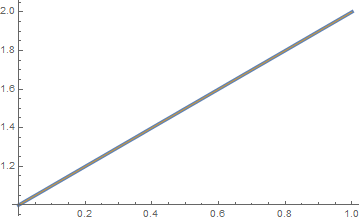
\includegraphics[height=7cm, width=10cm]{pics/0reconstruction.png}\\
	\caption{Porównanie początkowej funkcji granicznej z odtworzoną}
\end{center}
\end{figure}

Przygotowano również wykres pokazujący błąd bezwzględny obliczeń, co przedstawia poniższy rysunek: \\

\begin{figure}[H]
\begin{center}
		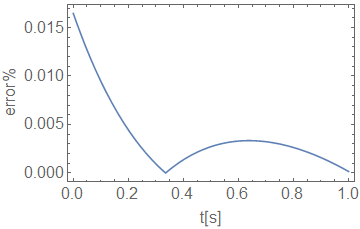
\includegraphics[height=7cm, width=10cm]{pics/0abs.png}\\
	\caption{Błąd bezwzględny obliczeń}\
\end{center}
\end{figure}

\subsubsection{1\% błąd pomiarowy temperatur}

Pomiary wykorzystywane przy obliczeniach z 1\% zakresem błędu pomiarowego wyglądają następująco: \\

\begin{tabularx}{\textwidth}{ | >{\rownum}c|X|} 
\hline
& \textbf{ $t_i$} \\ \hline
&0,8254\\ \hline 
&0,9273\\ \hline 
&1,0230\\ \hline 
&1,1173\\ \hline 
&1,2246\\ \hline 
&1,3169\\ \hline 
&1,4207\\ \hline 
&1,5227\\ \hline 
&1,6239\\ \hline 
&1,7363\\ \hline 
\end{tabularx}\\

Przeprowadzenie procesu odtwarzania funkcji granicznej dało następujące rezultaty (zaokrąglone do 4 miejsca po przecinku): \\

\begin{tabularx}{\textwidth}{ | >{\rownum}c|X|X|X|X|} 
\hline
& \textbf{Błąd} &
 \textbf{P} &
 \textbf{Q} &
 \textbf{S}\\ \hline
& 2,7209 * $10^{-2}$ & 0,1190 & 0,8952 & 1,0189 \\ \hline 
& 2,3787 * $10^{-2}$ & 0,1152 & 0,9157 & 1,0140 \\ \hline 
& 2,7362 * $10^{-2}$ & 0,1500 & 0,8860 & 1,0063 \\ \hline 
& 2,3056 * $10^{-2}$ & 0,1173 & 0,8890 & 1,0178 \\ \hline 
& 2,3617 * $10^{-2}$ & 0,1304 & 0,9021 & 1,0187 \\ \hline 
\end{tabularx} \\

Różnica pomiędzy oryginalną funkcją, a uzyskaną (poprzez u\si rednienie parametrów) została przedstawiona na wykresie: \\

\begin{figure}[H]
\begin{center}
		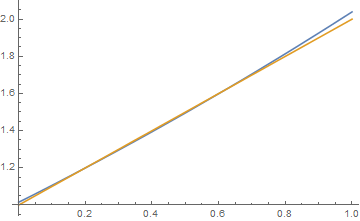
\includegraphics[height=7cm, width=10cm]{pics/1reconstruction.png}\\
	\caption{Porównanie początkowej funkcji granicznej z odtworzoną (z 1 \% zakresem błędu pomiarów)}
\end{center}
\end{figure}

Następujący rysunek przedstawia błąd bezwzględny obliczeń: \\

\begin{figure}[H]
\begin{center}
		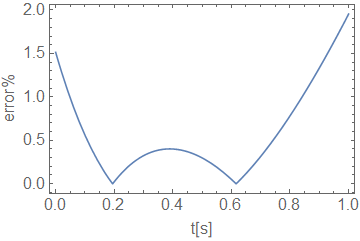
\includegraphics[height=7cm, width=10cm]{pics/1abs.png}\\
	\caption{Błąd bezwzględny obliczeń}
\end{center}
\end{figure}



\subsubsection{2\% błąd pomiarowy temperatur}

Przy obliczaniu parametrów odtwarzanej funkcji przy 2\% zakresie błędu pomiarowego wykorzystano następujące pomiary temperatur: \\
\begin{tabularx}{\textwidth}{ | >{\rownum}c|X|} 
\hline
& \textbf{ $t_i$} \\ \hline
&0,8327\\ \hline 
&0,9225\\ \hline 
&1,0161\\ \hline 
&1,1337\\ \hline 
&1,2405\\ \hline 
&1,3304\\ \hline 
&1,4376\\ \hline 
&1,5097\\ \hline 
&1,6126\\ \hline 
&1,6993\\ \hline 
\end{tabularx}\\ \newLine

Obliczone parametry wraz z błędem prezentują się następująco (przy zaokrągleniu do 4 miejsca po przecinku): \\

\noindent \begin{tabularx}{\textwidth}{ | >{\rownum}c|X|X|X|X|} 
\hline
& \textbf{Błąd} &
 \textbf{P} &
 \textbf{Q} &
 \textbf{S}\\ \hline
& 6,8528 * $10^{-2}$  & -0,3642 & 1,2993  & 0,9513 \\ \hline 
& 6,5422 * $10^{-2}$  & -0,2570 & 1,1971  & 0,9992 \\ \hline 
& 5,8742 * $10^{-2}$  & -0,2352 & 1,1853  & 0,9895 \\ \hline 
& 6,0410 * $10^{-2}$  & -0,1531 & 1,1175  & 0,9937 \\ \hline 
& 6,0850 * $10^{-2}$  & -0,1995 & 1,1643  & 0,9801 \\ \hline 
\end{tabularx} \\

Różnicę pomiędzy funkcjami pierwotną i obliczoną (poprzez u\si rednienie parametrów) przedstawia poniższy wykres: \\

\begin{figure}[H]
\begin{center}
		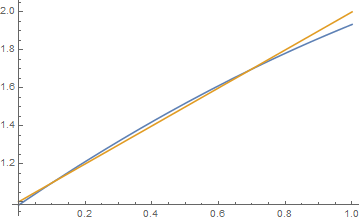
\includegraphics[height=7cm, width=10cm]{pics/2reconstruction.png}\\
	\caption{Porównanie początkowej funkcji granicznej z odtworzoną (z 2 \% zakresem błędu pomiarów)}
\end{center}
\end{figure}

Błąd bezwzględny obliczeń został przedstawiony poniżej: \\

\begin{figure}[H]
\begin{center}
		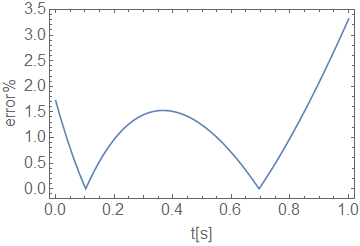
\includegraphics[height=7cm, width=10cm]{pics/2abs.png}\\
	\caption{Błąd bezwzględny obliczeń}
\end{center}
\end{figure}



\subsubsection{5\% błąd pomiarowy temperatur}

Pomiary wykorzystywane przy obliczeniach z 5\% zakresem błędu pomiarowego wyglądają następująco: \\
\begin{tabularx}{\textwidth}{ | >{\rownum}c|X|} 
\hline
& \textbf{ $t_i$} \\ \hline
&0,8051\\ \hline 
&0,9300\\ \hline 
&1,0515\\ \hline 
&1,1398\\ \hline 
&1,2139\\ \hline 
&1,2906\\ \hline 
&1,3880\\ \hline 
&1,5877\\ \hline 
&1,6267\\ \hline 
&1,7959\\ \hline 
\end{tabularx}\\

Wykorzystanie algorytmu dało następujące rezultaty (przy zaokrągleniu liczb do 4 miejsca po przecinku): \\

\noindent \begin{tabularx}{\textwidth}{ | >{\rownum}c|X|X|X|X|} 
\hline
& \textbf{Błąd} &
 \textbf{P} &
 \textbf{Q} &
 \textbf{S}\\ \hline
& 0,2031 & 0,8678 & 0,2034 & 1,1597 \\ \hline 
& 0,2049 & 0,6563 & 0,4295 & 1,0985 \\ \hline 
& 0,2030 & 0,7652 & 0,3167 & 1,1265 \\ \hline 
& 0,2060 & 0,8133 & 0,2428 & 1,1277 \\ \hline 
& 0,2041 & 0,7516 & 0,3426 & 1,1119 \\ \hline 
\end{tabularx}\\

Wykresy obu funkcji zostały przedstawione poniżej: \\

\begin{figure}[H]
\begin{center}
		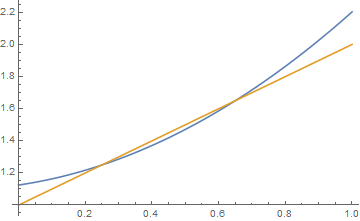
\includegraphics[height=7cm, width=10cm]{pics/5reconstruction.png}\\
	\caption{Porównanie początkowej funkcji granicznej z odtworzoną (z 5 \% zakresem błędu pomiarów)}
\end{center}
\end{figure}

Poniższy rysunek przedstawia błąd bewzględny obliczeń: \\

\begin{figure}[H]
\begin{center}
		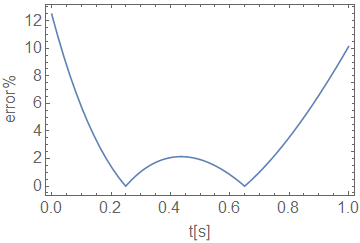
\includegraphics[height=7cm, width=10cm]{pics/5abs.png}\\
	\caption{Błąd bezwzględny obliczeń}
\end{center}
\end{figure}





\section{Podsumowanie}
Celem tej pracy inżynierskiej było stworzenie aplikacji, która pozwoliłaby rozwiązać zadany problem przewodnictwa ciepła poprzez zastosowanie algorytmu symulowanego wyżarzania. Stworzono więc program, który poprzez prosty interfejs graficzny pozwala na użycie tego algorytmu heurystycznego do wyznaczenia minimum w kilku funkcjach testowych oraz do rozwiązania zadanego odwrotnego zadania przewodnictwa ciepła. \\

Realizacja założeń projektu wymagała przeprowadzenia badań w kwestii odpowiedniego doboru parametrów dla poszczególnych problemów i ich jako\si ci oraz przetestowania i zoptymalizowania samego działania algorytmu symulowanego wyżarzania. Dobrane parametry dla poszczególnych problemów pozwalają na stosunkowo szybkie i poprawne znalezienie optymalnego rozwiązania danego problemu, a wyniki przeprowadzonych testów rozwiązania odwrotnego zadania przewodnictwa ciepła na zbliżone odtworzenie jednego z brakujących parametrów modelu matematycznego. \\

%
Napisać o tym, że implementacja algorytmu spowodowała trudno\si ci, ważne są detale, coś o wynikach.
%

\begin{thebibliography}{12}

% sym
\bibitem{0} http://iswiki.if.uj.edu.pl/iswiki/images/2/20/AiSD\_22.\_Symulowane \_wy\%C5\%BCarzanie\_\%28problem\_komiwoja\%C5\%BCera\%29.pdf [dostęp: 20 sierpnia 2018]

\bibitem{1} M. Duque-Anth, \textit{Constructing efficient simulated annealing algorithms}, [w:] ,,Discrete Applied Mathematics", 1997 nr 77/2, s. 139-159 Dostępny w Internecie: https://www.sciencedirect.com/science/article/pii/S0166218X96001321
[dostęp 20 sierpnia 2018]

\bibitem{2} http://wikizmsi.zut.edu.pl/uploads/archive/5/5e/20140303092223!OzWSI\_I\_S1\_W1.pdf
[dostęp: 25 sierpnia 2018]

\bibitem{3} http://www.wikizmsi.zut.edu.pl/uploads/e/eb/OzWSI\_I\_S1\_c1.pdf
[dostęp: 25 sierpnia 2018]

%funkcje testowe
\bibitem{4} https://en.wikipedia.org/wiki/Test\_functions\_for\_optimization\#Test\_functions\_for\_single-objective\_optimization [dostęp: 30 października 2018]

\bibitem{5} H. Abiyev, M. Tunay, \textit{Optimization of High-Dimensional Functions through Hypercube Evaluation}, Dostępny w Internecie:https://www.ncbi.nlm.nih.gov/pmc/articles/PMC4538776/
[dostęp: 13 listopada 2018]


%wstep i opis problemu[?]
\bibitem{6} F. Rothlauf, \textit{Optimization Problems}, [w:] \textit{Design of Modern Heuristics: Principles and Application}, wyd. Springer-Verlag Berlin Heidelberg, 2011, s. 7-44, ISBN 978-3-540-72961-7
Dostępny w Internecie: https://pdfs.semanticscholar.org/b333/0f96d1a937fc2c63b3294729cfea30826134.pdf
[dostęp: 27 listopada 2018]

%wstep i opis problemu
\bibitem{7} R. Martí, G. Reinelt, \textit{Heuristic Methods}, [w:] \textit{The Linear Ordering Problem, Exact and Heuristic Methods in Combinatorial Optimization}, wyd. Springer-Verlag Berlin Heidelberg, 2011, s. 17-40, ISBN 978-3-642-16728-7

%problemy odwrotne/1 rozdzial
\bibitem{8} http://prac.im.pwr.edu.pl/$\sim$plociniczak/lib/exe/fetch.php?media=odwrotne.pdf
[dostęp: 10 grudnia 2018]

\bibitem{9} https://www.math.unl.edu/$\sim$scohn1/8423/wellposed.pdf
 [dostęp: 10 grudnia 2018]

\bibitem{10}E. Hetmaniok, A. Zielonka, D. Słota, \textit{Zastosowanie algorytmu selekcji klonalnej do odtworzenia warunku brzegowego trzeciego rodzaju}, [w:] ,,Zeszyty naukowe Politechniki Śląskiej", 2012 nr 2/1874

\bibitem{11} E. Hetmaniok, D. Słota, A. Zielonka, \textit{Application of the Ant Colony Optimization Algorithm for Reconstruction of the Thermal Conductivity Coefficient}, [w:] \textit{Swarm and Evolutionary Computation}, wyd. Springer-Verlag Berlin Heidelberg,  2012,  s. 240-248, ISBN 978-3-642-29352-8


\end{thebibliography}
\end{document}